\documentclass[12pt,twoside]{article}
\usepackage{chadstyle}  % Loads my formatting 
\usepackage{longtable,booktabs}
\usepackage{stmaryrd}
%%%%%%%%\usepackage{mdframed}
\usepackage{titlesec}
\usepackage{hyperref}
%%%%%%%%%\usepackage{amsthm}

\usepackage{multirow}

\usepackage{glossaries}
\makeglossaries


\usepackage{bigints}
%%%%\usepackage[lite]{mtpro2}
\usepackage{physics}
\usepackage{scalerel}
\usepackage{mathrsfs}
\usepackage{empheq}

\usepackage{extarrows}
\usepackage{oubraces}

\usepackage{lmodern}
  \usepackage[T1]{fontenc}
  \usepackage[utf8]{inputenc}
  \usepackage{textcomp} % provides euro and other symbols
% use upquote if available, for straight quotes in verbatim environments
\IfFileExists{upquote.sty}{\usepackage{upquote}}{}
\usepackage{csquotes}

%\usepackage{tweaklist}  % I use this package as well; you may need to download

%% Shortcut commands

\usepackage[svgnames]{xcolor}%
\usepackage[amsmath]{ntheorem}
\usepackage[ntheorem]{mdframed}
\newmdtheoremenv[linewidth=5pt, linecolor=Gainsboro!75!Lavender, topline=false, bottomline=false, skipabove=15pt, skipbelow=20pt]{thm}{\color{ChadBlue}Théorème}

\newmdtheoremenv[linewidth=5pt, linecolor=Gainsboro!75!Lavender, topline=false, bottomline=false, skipabove=15pt, skipbelow=20pt]{lemme}{\color{ChadBlue}Lemme}

\newmdtheoremenv[linewidth=5pt, linecolor=Gainsboro!75!Lavender, topline=false, bottomline=false, skipabove=15pt, skipbelow=20pt]{definition}{\color{ChadBlue}Définition}


%   \theoremclass{Theorem}
%\newtheorem{proposition}{\color{ChadBlue} Théorème}
%\newtheorem{lemme}{\color{ChadBlue} Lemme}
%\newtheorem{definition}{\color{ChadBlue} Définition}

\newcommand{\Proof}[2]{{\hspace{-\parindent} {\color{ChadBlue}\bf Démonstration}~\ref{#1}.}
{#2}\hfill$\blacksquare$ \\ \vspace{.1in}}



%\newcosecnumdepthmmand{\proptitle}[1]{\color{ChadBlue} \textnormal{(#1):}}
%\newtheorem{proposition}{\color{ChadGreen} Proposition}
%\newcommand{\assume}[2]{{\bf{Assumption #1}} (#2)} 
%\newcommand{\clr}[1]{{\color{ChadBlue} #1}}
%\newcommand{\clrg}[1]{{\color{ChadGreen} #1}}
%\newcommand{\Proof}[2]{\newline {\hspace{-\parindent} {\color{ChadGreen}\bf Proof of Proposition}~\ref{#1}.}
%{\color{ChadBlue} #2} \vspace{.1in}}

% If you've loaded *tweaklist.sty* above, uncomment these lines:
% Adjust spacing in itemize/enumerate; see tweaklist.sty
%\renewcommand{\enumhook}{\setlength{\topsep}{2pt}%
%  \setlength{\itemsep}{0pt}}
%\renewcommand{\itemhook}{\setlength{\topsep}{2pt}%
%  \setlength{\itemsep}{0pt}}

\ifnum 0\ifxetex 1\fi\ifluatex 1\fi=0 % if pdftex
  \usepackage[shorthands=off,main=french]{babel}
\else
    % See issue https://github.com/reutenauer/polyglossia/issues/127
  \renewcommand*\familydefault{\sfdefault}
    % load polyglossia as late as possible as it *could* call bidi if RTL lang (e.g. Hebrew or Arabic)
  \usepackage{polyglossia}
  \setmainlanguage[]{french}
\fi

\providecommand{\tightlist}{%
  \setlength{\itemsep}{0pt}\setlength{\parskip}{0pt}}

\setcounter{secnumdepth}{4}
\setcounter{tocdepth}{3}

\titleformat{\paragraph}
{\normalfont\normalsize\bfseries}{\theparagraph}{1em}{}
\titlespacing*{\paragraph}
{0pt}{0pt}{0pt}
%{0pt}{3.25ex plus 1ex minus .2ex}{1.5ex plus .2ex}

\usepackage{setspace}
\setstretch{1.2}

%eviter les lignes blanches
\raggedbottom

%\newcommand*\widefbox[1]{\fbox{\hspace{2em}#1\hspace{2em}}}
\newcommand*\widefbox[1]{{\setlength\fboxsep{10pt}\fbox{\hspace{0.5em}#1\hspace{0.5em}}}}




%JEC
\DeclarePairedDelimiter\floor{\lfloor}{\rfloor}
\DeclarePairedDelimiterX{\Iintv}[1]{\llbracket}{\rrbracket}{\iintvargs{#1}}
\NewDocumentCommand{\iintvargs}{>{\SplitArgument{1}{,}}m}
{\iintvargsaux#1} %
\NewDocumentCommand{\iintvargsaux}{mm} {#1\mkern1.5mu..\mkern1.5mu#2}


\newcommand{\fcc}[1]{\widehat{#1}^{\raisebox{1pt}{\,\scriptsize$\ast$}}}
\usepackage{stackengine}
\stackMath
\def\hatgap{2pt}
\def\subdown{-2pt}
\newcommand\reallywidehat[2][]{%
\renewcommand\stackalignment{l}%
\stackon[\hatgap]{#2}{%
\stretchto{%
    \scalerel*[\widthof{$#2$}]{\kern-.6pt\bigwedge\kern-.6pt}%
    {\rule[-\textheight/2]{1ex}{\textheight}}%WIDTH-LIMITED BIG WEDGE
}{0.5ex}% THIS SQUEEZES THE WEDGE TO 0.5ex HEIGHT
_{\smash{\belowbaseline[\subdown]{\scriptstyle#1}}}%
}}
\begin{document}
%\bibliographystyle{aernobold}

%%%%%%%%%%%%%%%%%%%%%%%%%%%%%%%%%%%%%%%%%%%%%%%%%%%%%%%%%%%%%%%%%
% TITLE PAGE
%%%%%%%%%%%%%%%%%%%%%%%%%%%%%%%%%%%%%%%%%%%%%%%%%%%%%%%%%%%%%%%%%

\title{Notes sur le changement de repère}

%\runningheads{Sébastien Campagne}{Phénomène de Gibbs}

\author{Sylvie}
\date{\today}
\maketitle



%%%%%%%%%%%%%%%%%%%%%%%%
\begin{figure}
\centering
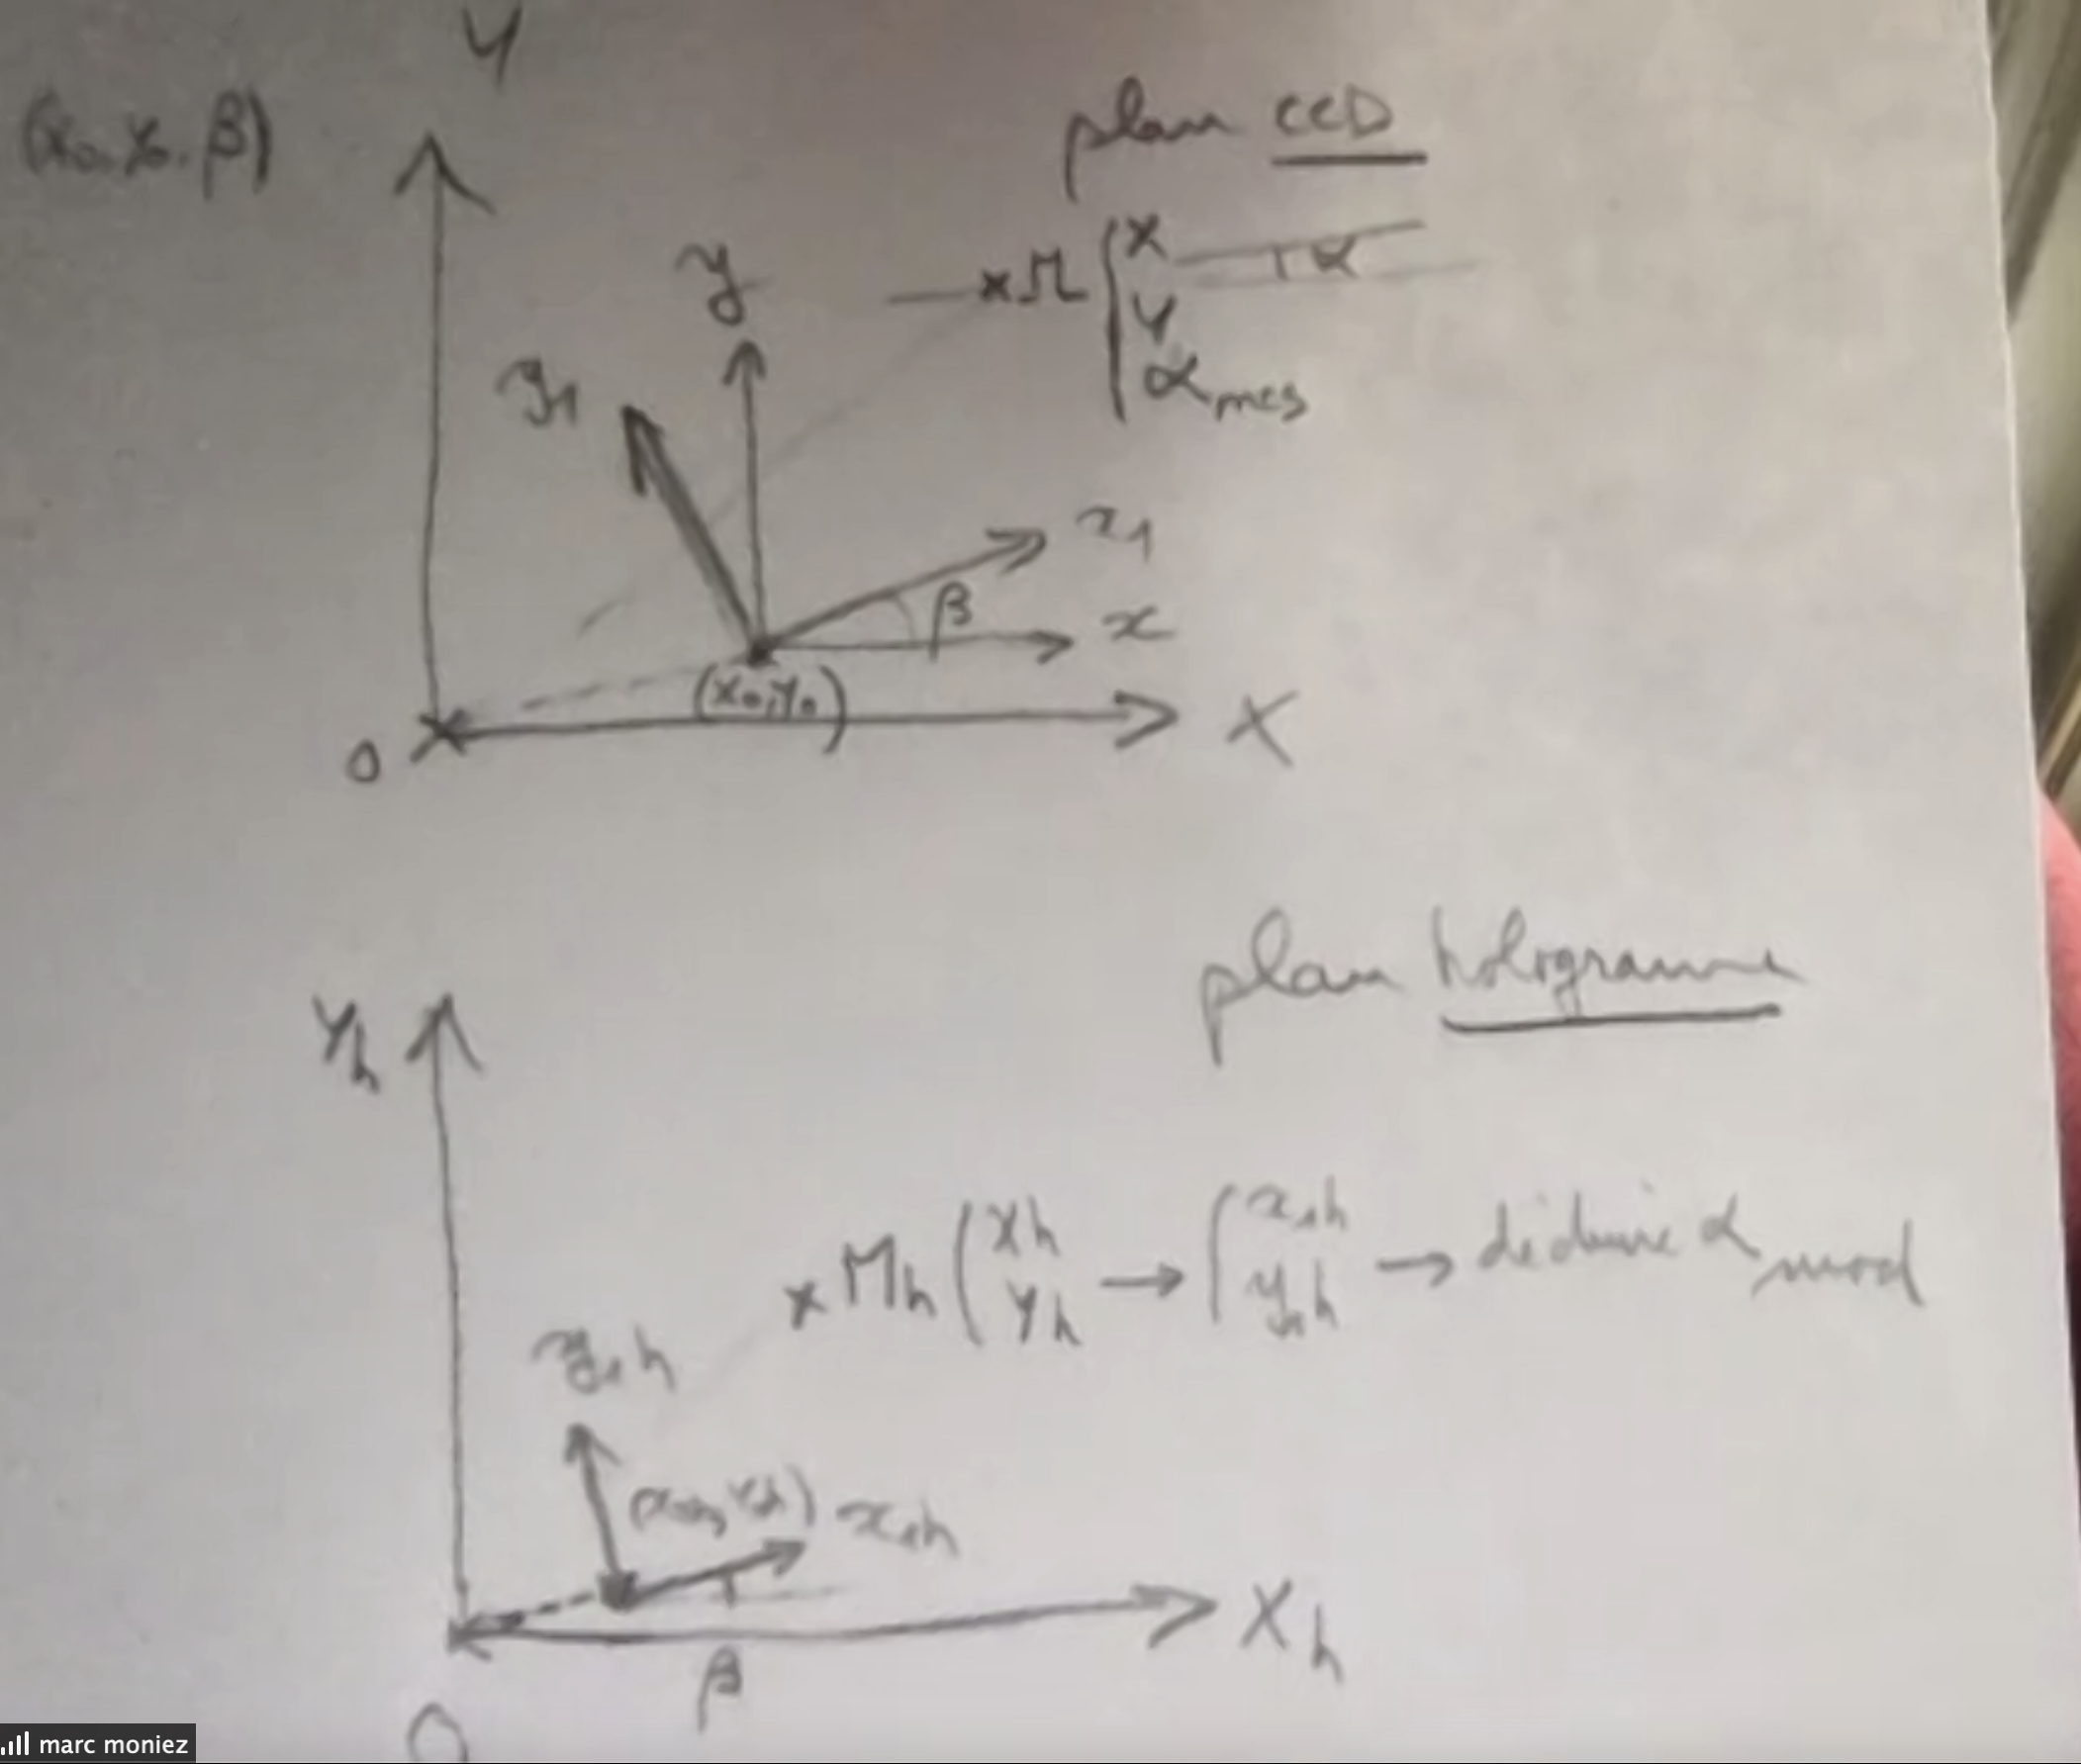
\includegraphics[width=0.8\textwidth]{Fig1.png}
\caption{Géométrie}
\end{figure}
%%%%%%%%%%%%%%%%%%%%%%%% 

On veut minimiser la fonction de $\chi^2(X_0,Y_0,\beta)$ définie ainsi:

\begin{equation}
 \chi^2(X_0,Y_0,\beta) = \sum_{i=1}^N \frac{\left( \alpha_{mes}^{(i)} - \beta - \alpha_{mod}(
 x^{(i)}_{1h},y^{(i)}_{1h})\right)^2}{\sigma_{\alpha}^{2, (i)}}
\end{equation}


où

\begin{itemize}
\item $(X_0,Y_0)$ sont les coordonnées du centre optique de l'hologramme $O_h$ dans le référentiel du CCD  dénoté ${\cal R }$ (par au centre optique du télescope $O$ et dont les axes coïncident avec les rangées et colonnes de pixels,
\item $\beta$ est l'angle de rotation du référentiel de l'hologramme ${\cal R}_{1h}$ défini au  point de coordonnées du point $O_h(X_0,Y_0)$  du centre optique dans le CCD, l'angle $\beta$ étant repéré par rapport aux axes de ${\cal R }$,
\item  $\alpha_{mes}^{(i)}$ est l'angle de l'axe de dispersion de l'ordre 1 d'une étoile,  mesuré dans le repère dans le repère ${\cal R }$ du CCD  et dont l'ordre 0 a pour coordonnées dans le CCD celles d'un point $M (X^{(i)},Y^{(i)})$ et les erreurs expérimentales sur la mesure des angles est $\sigma_{\alpha}^{(i)}$,
\item $N$ est le nombre de mesures, 
\item $ \alpha_{mod}( x^{(i)}_{1h},y^{(i)}_{1h})$ est l'angle de l'axe de dispersion à ce même point $M$ dans le référentiel dont les coordonnées dans le référentiel ${\cal R}_{1h}$   sont  $( x^{(i)}_{1h},y^{(i)}_{1h})$ et dont l'origine est prise au centre géométrique de l'hologramme $O_h$.

\end{itemize}

Pour des valeurs des paramètres $(X_0,Y_0,\beta)$ fixées les coordonnées $(x^{(i)}_{1h},y^{(i)}_{1h})$ du point $M$ dans ${\cal R}_{1h}$ sont calculables à partir des
coordonnées de ce point dans  ${\cal R}$~:
\begin{eqnarray}
x_{1h} & = & f_x(X,Y/X_0,Y_0, \beta) \\
y_{1h} & = & f_y(X,Y/X_0,Y_0, \beta) 
\end{eqnarray}

En négligeant pour simplifier des effets d'homothétie,
un point $M(X,Y)$ repéré dans  ${\cal R }$ a pour coordonnées $(x_h=X-X_0,y_h=Y-Y_0)$ repéré dans  ${\cal R }_{h}$ et donc a pour coordonnées dans  ${\cal R }_{1h}$~:

\begin{eqnarray}
x_{1h} & = & \cos \beta x_h + \sin \beta y_h \\
y_{1h} & = & -\sin \beta x_h + \cos \beta y_h 
\end{eqnarray} 

soit

\begin{eqnarray}
x_{1h} & = & \cos \beta (X-X_0) + \sin \beta (Y-Y_0) \\
y_{1h} & = & -\sin \beta (X-X_0) + \cos \beta (Y-Y_0)
\end{eqnarray} 


Pour vérifier si $\beta = \frac{\pi}{2}$,  on a bien $x_{1h}=y_h$ et $y_{1h}= -x_h$.

Inversement par rotation inverse,

\begin{eqnarray}
x_{h} & = & \cos \beta x_{1h} - \sin \beta y_{1h} \\
y_{h} & = & \sin \beta x_{1h} + \cos \beta y_{1h} 
\end{eqnarray} 

soit comme $(x_h=X-X_0,y_h=Y-Y_0)$~:

\begin{eqnarray}
X  & =  & X_0 +  \cos \beta x_{1h} - \sin \beta y_{1h} \\
Y  & = & Y_0 + \sin \beta x_{1h} + \cos \beta y_{1h} 
\end{eqnarray} 

\end{document}
